\chapter{Foundations: historical linguistics}
The purpose of this chapter is to give readers with a causal inference background sufficient knowledge of historical linguistics to arrive at a basic understanding of the new application domain. For readers with a linguistics background, it may serve as a quick overview of the relevant core definitions and issues of historical linguistics as I am framing them for the purpose of my work, sometimes deviating a little from the established terminology.

The second half of the chapter is of more interest to the linguist reader. It gives a rough overview of existing computational approaches to modeling language history, and discusses the current state of the art in reference to the methods of classical historical linguistics.

For the exposition, I need to presuppose some basic knowledge of phonology, or the sounds occurring in spoken languages. I will normally represent sounds by means of the IPA (International Phonetic Alphabet), which has become the standard across all branches of linguistics. To learn what these symbols represent, I recommend \citet{ladefoged_maddieson_1996}, the standard textbook of phonology. For readers who are not interested in languages and their pronunciation, but merely want to understand the methods I am developing and describing here, it should also be possible to follow the discussion by treating the IPA as a bag of elementary symbols (an alphabet in the formal sense), and not assigning any meaning or properties to them.

\section{Language relationship and family trees}
While very encompassing definitions of language can be given, at the core, a language such as English or Spanish can be seen as a system of symbols (vocabulary) and combination rules (grammar) used for communication. From this perspective, which is not shared by all traditions within linguistics, a language consists of a collection of symbols (lexical items\is{lexical item}, such as \textit{them}, \textit{give}, or \textit{renaissance}), and rules how these symbols can be combined (grammar rules, e.g.\ ``to combine an adjective with a noun, put the adjective in front of the noun'').

Obviously, individual languages can differ vastly in both the symbols they use and the grammar rules they use to recombine these symbols. While the sequences of sounds used to form the symbols are largely arbitrary and only constrained by limits on pronunciation and distinguishability, grammar rules in languages across the world show much more similarity in structure. The commonalities in the grammars of languages can be described in terms of typological features\is{typological feature}, such as the very basic fact whether adjectives usually precede the noun (as in \ili{English}) or follow the noun (as in \ili{Spanish}).

Just like most complex systems, human languages are constantly undergoing change. While some parts of a language change less quickly than others (e.g.\ words for body parts vs. slang terms), no part of a language is entirely immune to change. Over the course of millennia, changes will accumulate to the point were two languages which started out as dialects of the same language will end up having no recognizable similarities except the ones dictated by \textit{universals}\is{universal}, constraints on the structure of human language which are ultimately rooted in physiological or cognitive limits.

To give two concrete examples of language change, \ili{Old English} (OE) from about a thousand years ago, still distinguished different verb forms for the first and second person singular (\textit{ic stele} `I steal' vs. \textit{\th{}\={u} stilst} `you steal', cf. \textit{thou stealest} from about 500 years ago), and a boy was called \textit{cnafa}. Crucially, in addition to such instances of grammatical change and \isi{lexical replacement}, the phonetic shapes of words will invariably change over time due to \isi{sound change}. For instance, OE \textit{cnafa} \ipa{[knAvA]} became the modern word \textit{knave} \ipa{[neIv]}, where the [k] is not pronounced any more, and the \ipa{[A]} has been lengthened and then become a diphthong [\ipa{eI}].

For various external reasons, one (typically more isolated) part of a language community will sometimes not join in a change affecting the rest, or will undergo a change whereas the other speakers of the language do not. This is the prime mechanism by which a language can split into \textit{dialects}\is{dialect}, loosely defined as mutually comprehensible, but different variants of the same language. As time goes on, dialects tend to diverge further from each other, up to the point where their speakers do not understand each other any longer, which is when we start to call the former dialects separate languages. Since mutual comprehensibility is a continuum, and the comprehensibility relationship is not transitive (there can be dialect continua\is{dialect continuum} where each dialect remains comprehensible to its neighbors, but dialects which are farther apart are different languages), the definition of what we call a dialect and what a language is often arbitrary and not subject to linguistic criteria.

If we trace the development of one language as it recursively splits up into new variants through the ages, we arrive at a tree-shaped pattern which is called a \isi{phylogenetic tree}. As an illustration, Figure \ref{germanic-tree} visualizes how various \ili{Germanic languages} are reconstructed as having developed out of a common ancestor language, Proto-Germanic. The height dimension of the tree roughly represents the time dimension, and builds on the estimated \isi{time depth} of each intermediate stage, i.e.\ the time at which the respective proto-language is assumed to have split into its daughter languages. Some estimation of time depth is necessary for all advanced methods of phylogenetic inference, but it is a hotly contested topic because none of the methods for estimating time depth has led to full agreement with the known history of families where proto-languages are attested by written records. Today, historical linguists typically avoid talking about chronology (``linguists don't do dates''), 
due to a long history of premature conclusions which later turned out to be mistaken. Still, in the case of Germanic languages, there are sufficient historical records of many languages that the dates implied by the vertical dimension of the tree are widely considered as very likely.

\begin{figure}[hp!]
 \centering
 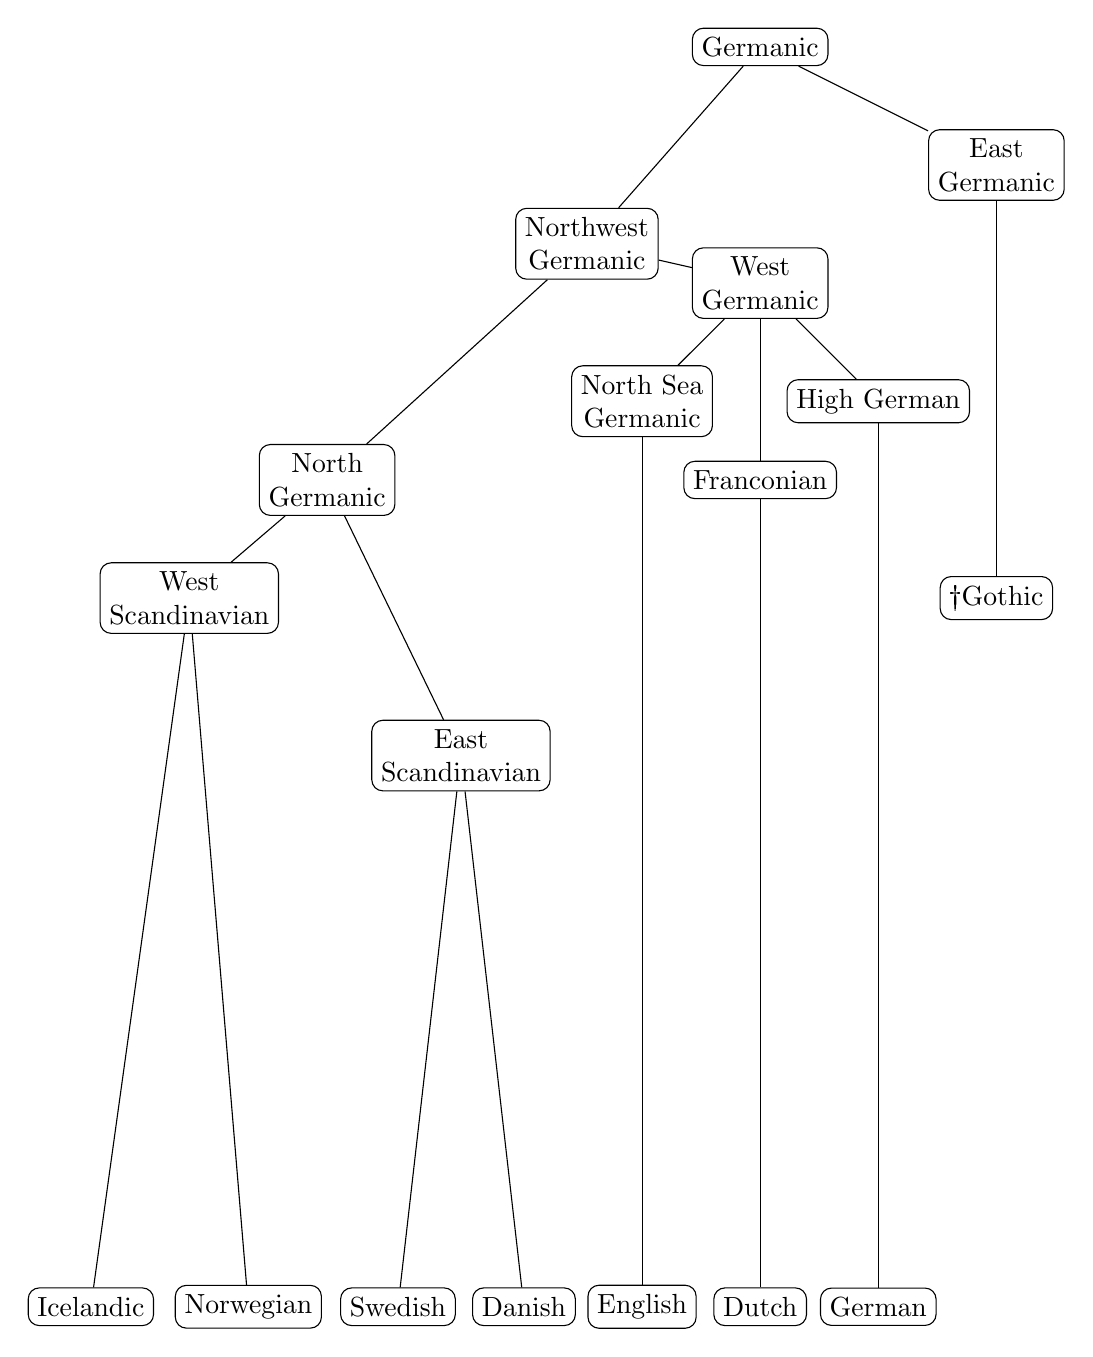
\begin{tikzpicture}[
  every node/.style = {shape=rectangle, rounded corners,
    draw, align=center,
    top color=white, bottom color=white}]]
  \node (G) at (8,16) {Germanic};
  \node (NWG) at (5.8,13.5)  {Northwest\\ Germanic};
  \node (NG) at (2.5,10.5) {North\\ Germanic};
  \node (WSc) at (0.75,9) {West\\ Scandinavian}; 
  \node (isl) at (-0.5,0) {Icelandic};
  \node (nor) at (1.5,0) {Norwegian};
  \node (ESc) at (4.2,7) {East\\ Scandinavian}; 
  \node (swe) at (3.4,0) {Swedish};
  \node (dan) at (5,0) {Danish};
  \node (WG) at (8,13) {West\\ Germanic};
  \node (NSG) at (6.5,11.5) {North Sea\\ Germanic};
  \node (eng) at (6.5,0) {English};
  \node (Frc) at (8,10.5) {Franconian}; 
  \node (nld) at (8,0) {Dutch};
  \node (HG) at (9.5,11.5) {High German}; 
  \node (deu) at (9.5,0) {German};
  \node (EG) at (11,14.5) {East\\ Germanic};
  \node (got) at (11,9) {\dag Gothic};
  
  \draw (G) -> (NWG);
  \draw (NWG) -> (NG);
  \draw (NG) -> (WSc);
  \draw (WSc) -> (isl);
  \draw (WSc) -> (nor);
  \draw (NG) -> (ESc);
  \draw (ESc) -> (swe);
  \draw (ESc) -> (dan);
  \draw (NWG) -> (WG);
  \draw (WG) -> (NSG);
  \draw (NSG) -> (eng);  
  \draw (WG) -> (Frc);
  \draw (Frc) -> (nld);
  \draw (WG) -> (HG);
  \draw (HG) -> (deu); 
  \draw (G) -> (EG);
  \draw (EG) -> (got);
  
\end{tikzpicture}
 \caption{A (partial) phylogenetic tree of Germanic languages}
 \label{germanic-tree}
\end{figure}

Languages which are descendants of the same proto-language are said to belong to the same \textit{\isi{language family}}. In practice, which languages are grouped together actually depends on whether the relationship between them has been proven. A family is thus not different in nature from any of its subgroups defined by a common proto-language, but whether we call it a family depends on the current state of our knowledge. The current partition of the world's languages into about 400 families (about half of these with only a single member) has however turned out to be remarkably stable for decades, indicating that the field might find itself near to a maximum time depth where enough similarites survive to prove genetic relationship. This maximum time depth is commonly assumed to lie between 6,000 and 8,000 years ago, with older relationships provable in the presence of old written records (as in the case of Afro-Asiatic\il{Afro-Asiatic languages}, a family with a time depth of about 10,000 years which 
includes ancient languages such as \ili{Hebrew}, \ili{Akkadian}, and \ili{Ancient Egyptian}).

Within the Indo-European language\il{Indo-European languages} family, the \ili{Germanic languages} form a \textit{\isi{taxon}}, i.e. a group of more closely related languages which in turn have a common ancestor. Often, families can be decomposed rather cleanly into several such taxa, whereas the question which taxon split off first is often difficult to answer and forms a large part of the debate among experts in the respective language family. The established taxa frequently correspond to a time depth of around 2,000 years, when the similarities between descendant languages are usually still so pervasive that the relationship is obvious to a layman taking a first glance at the basic vocabulary. For instance, it is quite obvious that \ili{English} \textit{wife}, \ili{German} \textit{Weib}, \ili{Dutch} \textit{wijf}, \ili{Swedish} \textit{viv}, and \ili{Icelandic} \textit{víf} are essentially the same word, and a dozen of these close parallels in basic vocabulary would be enough to define Germanic as a taxon.
 In contrast, proving that \ili{Armenian} \textit{kin}, \ili{Russian} \textit{žena}, \ili{Irish} \textit{bean}, \ili{Icelandic} \textit{kona}, and \ili{Persian} \textit{zan} are related in very much the same way, requires a lot more effort and expert knowledge, which is similar to the situation in many other families.

\section{Language contact and lateral connections}
What complicates the picture of neat family trees depicting in which order the languages of a family split off, is that languages are in contact\is{language contact} with each other, and that linguistic features do not only result from inheritance or random change, but also from \isi{borrowing} between languages which are in contact. To the non-linguist reader, the term \textit{borrowing} might seem slightly odd because the element taken from the donor language is never given back in any sense, in which case it helps to mentally equate borrowing with the copying of material. On the lexical level, a loan or \isi{loanword} is a word which gets copied by one language (the \isi{recipient language}) from another (the \isi{donor language}).

\ili{English} is a very good language for finding examples of contacts, as it represents a very interesting mix of inherited (Germanic) and borrowed (mostly Romance) features. On the level of morphology, English features two competing strategies of forming the comparative degree of an adjective, the Germanic suffix \textit{-er} as in \textit{larger} or \textit{thicker}, and the Romance-style pattern with \textit{more} as in \textit{more interesting} or \textit{more relevant}. The English lexicon is split roughly in half \citep{finkenstaedt_wolff_1973}, where the first half is dominated by basic vocabulary and words for everyday items and phenomena, which are typically either inherited from Proto-Germanic (\textit{eye}, \textit{rain}, \textit{hammer}) or borrowed from other \ili{Germanic languages} (\textit{window}, \textit{wing}, \textit{skin}). The other half mainly consists of terms of science and culture (\textit{science}, \textit{pious}, \textit{ignition}), all of which were borrowed from \ili{Latin} and 
\ili{Romance languages}. The convention is to consider the descent of the basic vocabulary and grammatical features as the relation defining the tree (and thereby the family membership), and to treat contact of any intensity as a secondary phenomenon, which makes English a Germanic rather than a Romance language.

Still, the sometimes very visible effects of language contact have always caused an undercurrent of historical linguistics to reject the tree model. Given the ubiquity of language contact, the underlying assumption of the tree model that languages continue to evolve independently after each split, and treating continued contact as the exceptional case, might seem unnatural. People in this school of thought have tended to adhere to an alternative \isi{wave model}, which is based on the observation that linguistic innovation tends to spread from a center to the periphery. Sometimes, innovations will sweep across language boundaries in situations of language contact, which then leads to borrowing. A language split occurs when a series of waves does not sweep across an entire language community. \citet{francois2014} provides a good recent overview of the theory behind wave models, and argues why they are attractive for describing some patterns of innovation. While generally accepted as well-suited for explaining areal phenomena and dialect continua, the strong assumption of wave-model advocates that any apparently tree-like signal in language evolution arises out of a pattern of overlapping waves is not advocated by many historical linguists any longer. While this view was once very popular due to certain phenomena in the history of Indo-European, it has been weakened by the abundance of quite clearly tree-like patterns in language families since studied. From the perspective of inference, wave models are problematic as well. The problem is that they have little explanatory value in the individual case, since every observable situation can be explained by many more different sequences of waves than sequences of splitting events which generate trees.

\section{Describing linguistic history}
Historical investigations about any given language often amount to proposing etymologies\is{etymology} for words. An etymology is a description of a word's history, typically featuring either the information which word in a reconstructed proto-language it evolved from, from which other language it was borrowed, or how it was derived from lexical material which already existed in the language. For instance, the etymology of the \ili{English} word \textit{house} is given by \cite{kroonen2013} as inherited from a reconstructed Proto-Germanic word \textit{*hūsa-}, which in turn is of obscure origin, although it might derive from a Proto-Indo-European root \textit{*kuH-} `to cover', which would connect the word to e.g. \ili{Latin} \textit{cutis} `skin' and \ili{Lithuanian} \textit{kiautas} `shell, rind, skin'. The etymologies one can establish thus vary in time depth, and tracing a word's history further into the past is a frequent type of contribution which would in this case advance our knowledge of Germanic. 
Etymological dictionaries for a single modern language will often include much more information about additional senses and when they developed, as well as the first attestations of some idioms involving the headword. This type of information is not required for the word to have an etymology, and most etymological dictionaries do not include such information, often due to a lack of historical data.

In classical historical linguistics, words which are derived from the same word in a common proto-language are called \textit{cognates}\is{cognate}, whereas borrowed words and their descendants are not counted as belonging to the same \isi{cognacy class}.
While the clean separation of inherited words and loanwords is crucial to the classical method, computational methods have tended to put less emphasis on this distinction. This leads to a somewhat unfortunate difference in terminology between classical and computational historical linguistics, as the latter customarily subsumes both inheritance and borrowing under the cognacy relation. As an alternative term to cover this more liberal notion of cognacy, \textit{correlate} has some currency, but I opt not to use it here because of the otherwise confusing frequent occurrence of the concept of correlates in the statistical sense in the text. Instead, I will use \textit{\isi{true cognacy}} for the stricter classical sense whenever the distinction is relevant, and otherwise stick to the more liberal usage established in computational historical linguistics.

Expanding on the basic distinction of inherited items and loans in a language's lexicon, descriptions of loanwords are usually more fine-grained. Very often, loanwords of roughly the same age from the same donor languages can be grouped into strata\is{stratum} or layers. For instance, there is a rather thin stratum of Celtic\il{Celtic languages} loans in \ili{English}, which includes words such as \textit{basket}, \textit{beak}, and \textit{nook}. This Celtic stratum can be further subdivided into an \ili{Ancient Brittonic} layer (to which the mentioned words belong), and later borrowings from languages such as \ili{Welsh} (\textit{bard}, \textit{crag}) and \ili{Irish} (\textit{galore}, \textit{slogan}). In effect, the lexicon of every language can be split into an inherited core vocabulary, and a number of loanword strata which came into the language at different times from different languages.

\section{Classical methods}
This section provides a concise introduction into the mindset and the methods of classical historical linguistics, the discipline to which we owe the bulk of our current knowledge about the history of the world's languages, and against the results of which computational methods are commonly evaluated. Historical linguistics is a much broader field than a short introduction to core principles would suggest, and the non-linguist reader is encouraged to explore the field in its breadth by means of a handbook, such as the excellent recent one by \citet{bowern_evans_2015}.

\subsection{The comparative method}
The primary tool of historical linguistics is the \textit{\isi{comparative method}}, a well-tested set of principles which has been developing for about two centuries, and has proven its worth as a tool for reconstructing the history of many language families. The key idea is to build on the assumed (and rather robustly attested) regularity of sound changes to reduce the likelihood that observed similarities between words from different languages are only due to chance. For a group of languages, relationship is then proven by reconstructing the sound inventory and the phonetic shape of many words in an assumed common proto-language, and then explaining how the known forms in each descendant language evolved from their equivalent in the proto-language by a series of regular sound changes.

\subsubsection{Sound correspondences}
On the synchronic level, both inheritance and regular sound changes lead to recurring sound correspondences in cognate words. For instance, there is a fairly regular sound correspondence between word-initial \ili{English} \textit{p} \ipa{[p\textsuperscript{h}]} and \ili{German} \textit{pf} \ipa{[\t{pf}]}, as evidenced by pairs like \textit{pan/Pfanne}, \textit{plum/Pflaume}, and \textit{pluck/pflücken}. The last two examples show that we cannot expect one-to-one correspondences across all comparable segments in cognate pairs: English \textit{u} \ipa{[2]} can apparently correspond to German \textit{au} \ipa{[A\textsubarch{U}]} or \textit{ü} \ipa{[Y]}. The reason for such a one-to-many correspondence can be either that two different phonemes have merged into English \ipa{[2]}, or that one proto-phoneme diverged into the two German variants due to a conditional sound law, i.e.\ a change which happened regularly in a specific phonological context, which might have left no traces in the observable forms.

\subsubsection{Sound laws}
In the Neogrammarian view, the sound correspondences between related languages are the result of \textit{sound laws}\is{sound law}, i.e.\ regular phonetic changes which occurred while the languages developed from their common proto-language. In the simplest case, a sound change replaces all occurrences of some sound by a different one. However, in reality, sound laws almost never occur unconditionally, i.e.\ they will typically only apply in a certain phonetic context (such as between vowels, or in stressed syllables). Due to this context dependency, sound changes can increase the number of phonemes in a language, whereas unconditional rules could only keep the number of phonemes constant (if the resulting phoneme was not present in the language before), or decrease it (if two phonemes merge). For instance, the phoneme \ipa{[\t{tS}]} that is written \textit{ch} in modern \ili{English}, did not exist in West Germanic, and only developed during the Anglo-Frisian stage in a rather common process called 
palatalization, where velar plosives become palatals (often affricates) under the influence of adjacent front vowels. In other contexts, ancestral \ipa{[k]} was left untouched. This explains the seemingly irregular sound correspondence between English \textit{choose} (\ili{Old English} \textit{ċēosan}) and \ili{Dutch} \textit{kiezen}, whereas we have \ipa{[k]} in both English \textit{cat} and its Dutch cognate \textit{kat}.

The crucial idea of the Neogrammarian school of linguists is that such sound laws apply without exception, i.e.\ they apply to all instances of a sound in a particular context throughout the words of a language. These contexts can be quite complex, as can quickly be demonstrated using \ili{English} and \ili{German}. The sound law which produced the mentioned \textit{p/pf} correspondence between English and German is part of the second phase of the High German consonant shift. By comparing the contexts in which this correspondence as well as analogous instances of affricatization (\ipa{[t]} $\rightarrow$ \ipa{[\t{ts}]} and \ipa{[k]} $\rightarrow$ \ipa{[\t{kx}]}) occur, one finds that the law must have applied in four distinct contexts: word-initially, when geminated (\ipa{[p:],[t:],[k:]}), after liquids (\ipa{[l]} and \ipa{[r]}), and after nasals (\ipa{[m]} and \ipa{[n]}). For the \textit{p/pf} pair, we have already seen examples of the first context. Instances of the second context are \textit{apple/Apfel} and \textit{copper/Kupfer}. The liquid context is exemplified by \textit{carp/Karpfen}, and as examples of the nasal context we have \textit{swamp/Sumpf} and \textit{cramp/Krampf}. This pattern reliably repeats itself across all the lexical material which both languages inherited from West Germanic.

Since sound changes are historical events which happen during a short timeframe, the laws which shaped the history of a language can be arranged into a sequence in which they occurred. Because sound laws frequently interact (e.g.\ if one change creates a context where the next law can apply), we can often derive constraints on the possible order in which they must have occurred, leading at least to a partial relative chronology. For instance, we know that the third stage of the High German consonant shift, which in some \ili{German} dialects turned voiced plosives into voiceless ones (e.g.\ \textit{[b]} $\rightarrow$ \textit{[p]}, must have occurred after affricatization, because the voiceless stops would otherwise have become affricatized in turn. We can exlude this order of events based on the fact that the German cognate of English \textit{bread} is not \textit{*Pfrot}, but \textit{Brot}, which is pronounced something like \ipa{[pRo:t]} in the dialects which underwent the third stage of the shift.

While we frequently can derive constraints on the relative order of sound changes in this way, an absolute chronology of sound changes is much more difficult to derive. Typically, it is necessary to rely on historical knowledge or written sources for this. For instance, we know for certain that the High German sound shift must have happened before the 8th century, because \ili{Old High German} texts from that time already display the results of that change. For written languages where we have no written sources in scripts which reveal the phonology, a (partial) relative chronology is often the best we can arrive at.

\subsubsection{Distinguishing inherited words from loans}
The work of establishing sound changes and their chronology is necessarily based on reflexes of the same proto-words across descendant languages. The groundwork of historical linguistics has therefore always revolved around the tasks of finding true cognates, distinguishing them from loans, and separating the loanwords in each language neatly into strata. This sometimes very complicated task forms the necessary preparatory work for later higher-level steps such as determining isoglosses, and reconstructing proto-languages in order to establish phylogenetic units.

In addition to reducing the likelihood of words becoming similar due to chance, the regularity of sound change also provides us with the most important source of hints about the etymology of words, especially when deciding whether some word was inherited, or borrowed from a sister language. For instance, the Proto-Germanic shift from [k] to [h] is enough to prove that \ili{Latin} \textit{cellarium} `pantry' and \ili{German} \textit{Keller} `cellar' cannot be true cognates, because we would expect something like \textit{*Heller} in this case. Although interactions between sound laws, and gaps in our knowledge about them, can make this type of argument quite complex, it is typically possible to recognize non-cognates, and estimate the time at which they were borrowed, for a large portion of a language's basic lexicon.

\subsubsection{Reconstructing ancestral forms}
With cognate sets and sound laws established, in theory it should become an almost mechanical task to project the attested words back to reconstructed proto-forms by reverse application of the sound laws. If this back-projection does not lead to the same proto-form if we start from different descendant languages, this is a hint that some of our current hypotheses about sound laws and cognacy relations must be wrong, and provides us with clues about the ways in which our theory needs to be revised.

In practice, there are many phenomena which complicate the picture, and make reconstruction of ancestral forms a non-trivial task. The most pervasive of these is \textit{analogy}, which subsumes a variety of very frequently occurring phenomena by which irregular changes can happen whenever the result becomes in some way easier to represent and process than the initial form. To quote two of the many examples given by \cite{campbell1999} in his introduction to historical linguistics, the vowel contrast between the \ili{English} adjective \textit{old} and its old comparative form \textit{elder} (which still survives in \textit{elder brother}) became leveled to yield current \textit{older}, and \ili{German} \textit{Natter} is cognate with English \texttt{adder}, which lost its initial \textit{n} due to reanalysis of its combination with the indefinite article, such that \textit{a nadder} became \textit{an adder}.

To give another more complex example from a different language family, the Proto-Uralic\il{Uralic languages} words \textit{*ükte} and \textit{*kakta} are one possible reconstruction for the numbers `one' and `two'. The latter should have resulted in \ili{Finnish} \textit{*kahda-} by regular sound change, but the actual form is \textit{kahde-}. In contrast, Finnish \textit{yhde-} `one' is the completely regular result of applying known sound laws to \textit{*ükte}. It is generally assumed that the irregular form \textit{kahde-} received its final vowel by analogy, making the words for the two numbers more similar. The decision that \textit{*kakta} and not \textit{*ükte} is the word that was reshaped is necessarily based on reflexes in other branches of Uralic, which demonstrates why analogy complicates reconstruction. In fact, because irregular changes also appear to have happened to \textit{*kakta} in other branches of Uralic, there is still no consensus whether \textit{*kakta} is actually the correct 
reconstruction.

Explanations involving analogy are very common in etymological research, and it seems that analogy is a force just as important as regular sound change in shaping words. For historical linguistics, relying too much on analogy when explaining word forms is quite risky, because allowing almost arbitrary sporadic changes to apply to only one or a few words makes it much easier to fit forms to any reconstructions, detracting from the strength of the method.

\subsubsection{Establishing phylogenies}
By reconstructing ancestral proto-forms for a set of cognates in a set of attested languages, and proving that the regular sound changes and additional assumptions such as analogies correctly generate the different attested forms from the reconstructed form, a historical linguist proves that the attested languages form a phylogenetic unit. By reconstructing older proto-languages as common ancestors of already established younger ones, it should in principle be possible to establish the entire phylogenetic tree of a language family, detailing in which order various genera split off the common proto-language, and how these in turn split into the attested languages.

If we continue this reconstruction process through the ages, shouldn't it be possible to trace the history of each language back to very few large families? If one assumes \textit{monogenesis}, i.e.\ that human language has only developed once, and not independently in different places, one could even imagine deriving a world tree, detailing how the modern human languages developed out of a single ancestral language of humankind.

Unsurprisingly, there are limits to the comparative method preventing us from getting this far. The more sound changes accumulate through the ages (especially under complicated conditions), the more indistinguishable the inherited similarities will be from chance similarities. To still isolate individual sound laws and unravel in which contexts and in which order they applied, we would need ever larger numbers of cognacy candidates. The most serious limitation for the method therefore lies in the fact that cognate density actually decreases. Due to semantic change, lexical replacement, and borrowing, the cognates shared between two related languages are bound to get lost with time. Since every language has only a finite number of basic lexemes, already after a few millennia the languages will cease to share enough cognates for regular sound correspondences to be established, and the comparative method ceases to work.

For well-documented language families, the limits of the comparative method in terms of establishing deep ancestry appear to have been reached quite some time ago. What is more, many families which are generally considered established (such as Afroasiatic, and Sino-Tibetan) are not proven as genetic units in the strict sense, as there are no single widely accepted reconstructions of the respective proto-languages. The maximum age of phylogenetic units which can still be safely established using the comparative method seems to lie at between 6,000 and 8,000 years before present, which leads us far into prehistory in most parts of the world, but is a far cry from being able to get back to the times when e.g.\ the Americas or Australia were settled. Any method which tries to answer questions at higher time depths based on language data will need to resort to statistical arguments, or typological similarities, both of which cannot rule out the possibilities of chance similarity (a risk which is high for 
typological variables due to universals) and ancient contact.

\subsubsection{Shared retentions and innovations}
But the methodological limits of the comparative method do not only appear at high time depths, but also when making family-internal classification decisions. To reliably separate one taxon from the rest of the family, the amount of lexical overlap in terms of shared cognates is considered an insufficient criterion. Even if we excluded the possibility of borrowing, a larger-than-average lexical overlap between two languages we want to group together can still be either due to shared retentions (the languages outside the group under consideration changed) or shared innovations (the change happened from the proto-language of the family to the taxon we are trying to establish). The existence of correspondences alone does not yet allow us to decide whether we are dealing with shared retentions or innovations. The main reason why many subgroupings which seem obvious on a lexical level are sometimes not generally accepted is that quite often, the hypothetical common proto-language is so close to the proto-language 
of the entire family that no regular changes can be detected to define the transition between the two proto-languages. The requirement of demonstrable shared innovations often severely limits the ability of classical historical linguists to clarify the internal structure of a language family beyond the level of securely established branches.

\subsection{Theories of lexical contact}
Whenever speakers of two different languages get in intensive contact with each other, this will invariably leave traces in those languages. According to \citet[Section 8.5]{hock_joseph_1996}, the main variable deciding about the shape of lexical influence between two languages is the difference in prestige. This difference is the standard explanation for the fact that languages do not only borrow needed words for new concepts (such as \ili{German} \textit{Computer} and \textit{Internet}), but also tend to replace perfectly workable and well-established terms for some concepts with those from a prestige language (German \textit{Service} instead of \textit{Dienstleistung}, or \textit{Ticket} instead of \textit{Fahrkarte}).

As \citet{thomason_kaufman_1988} elaborate in their analysis of contact situations, the decisive factor determining how a contact situation between a high-prestige and a low-prestige language plays out is whether it occurs under conditions of maintaining the low-prestige language, or language shift towards the high-prestige language. The first scenario will typically lead to a situation of widespread bilingualism, where even words for basic concepts tend to be replaced by their borrowed equivalents, as the familarity of the bilinguals with the higher-prestige language increases at the expense of the lower-prestige recipient language. The situation where the prestige gradient is not too high, and both languages continue to coexist for many generations, is the one where one would expect the largest amount of borrowings even of basic vocabulary items. The words borrowed from a language of comparable prestige are said to form an adstratum. For instance, \ili{English} has a North Germanic\il{North Germanic languages} 
adstratum from the time when the Vikings settled large parts of England, and started to intermarry with the local population. Words borrowed by English during this time include very basic vocabulary items such as \textit{to take} and \textit{they}.

In the second scenario, the target language is learned imperfectly by shifting speakers, which tend to retain many phonological and syntactic features of the original language, but typically not much lexical material except terms for local plants and animals. If the number of shifting speakers is demographically relevant, the structural \isi{substrate} influence will result in a changed variant of the target language. A case in point is the Western Uralic substrate in \ili{Russian} which shows itself in certain syntactic features which set Russian apart from its Slavic sister languages, such as the lack of a copula in the present tense, and the extensive use of the partitive genitive.

In the case where both languages are maintained (i.e.\ in the absence of language shift), \citet{thomason_kaufman_1988} distinguish five degrees of contact intensity, each with characteristic manifestations in the extent of lexical and structural borrowing. The first three stages represent different degrees of lexical borrowing, with accompanying weak structural borrowing that does not cause any shifts in the typological profile. Under circumstances of casual contact, we would only expect content words to be borrowed, and typically non-basic vocabulary. Under slightly more intense contact, conjunctions and adverbial particles will be among the first structural elements which are taken over. Only under very intense contact will we observe borrowing of other function words such as adpositions, pronouns, and low numerals. Bound morphemes such as derivational affixes may also be transferred at this stage, and they can stay functional in the borrowing language. The last two stages describe situations of strong 
and very strong cultural pressure, where the structural influence is so strong that typological changes can occur. On the lexical level, contact of this intensity will lead to massive borrowing which can even replace large parts of the basic vocabulary.

\subsubsection{Types of borrowing}
In the bilingual environment where most lexical borrowings occur, a loanword is initially borrowed in its original phonetic shape. With time, loans tend to get nativized by sound changes, often up to a point where they are not recognizably foreign any longer. An instance of this is \ili{German} \textit{Fenster} `window', which was borrowed from \ili{Latin} \textit{fenestra} into \ili{Old High German}, i.e.\ more than a thousand years ago. Without knowledge of Latin, no native speaker of German would suspect that this word was not inherited from the parent language. By contrast, more recent loans in German, such as \textit{E-Mail} from \ili{English}, tend to contain sounds foreign to German (the diphthong \ipa{[eI]}), or to deviate from the usual orthographic rules (the long vowel \ipa{[i:]} written as \textit{e}, instead of \textit{ie} or \textit{ih}), and are therefore instantly recognized as loanwords.

While from the perspective of cognacy, borrowing across families will tend to be detectable as words from a different cognate class, the quite common situation of \isi{internal borrowing} within the same language family often leads to a word getting replaced by a cognate word from a sister language. For instance, this is what happened with the \ili{English} word \textit{guard}, which replaced older \textit{ward} by a cognate borrowed from \ili{Frankish} via \ili{French}, where a regular sound change from \ipa{[w]} to \ipa{[g]} had occurred (cf. \textit{William} vs. \textit{Guillaume}). Both cross-family and family-internal borrowing will commonly happen whenever living languages come into close contact.

A lot less frequently, words can also be borrowed from ancient languages, which might even be direct ancestors of the recipient language. This tends to happen with high-prestige written languages that persist as languages of religion or science. The most well-known examples are Latin in Western and Southern Europe, from which \ili{Romance languages} did not only inherit, but also borrow words, and \ili{Sanskrit}, which plays the same role across India. Less well-known examples of the same pattern include \ili{Old Church Slavonic}, from which many words were borrowed into later East Slavic languages such as Russian, and the influence of \ili{Pali}, the Middle Indo-Aryan language of Theravada Buddhism, on many languages of Southeast Asia. If a language borrows from its own ancestor or a close relative, this very frequently leads to doublets like the \textit{guard/ward} example, which are also called etymological twins. For instance, the Latin word \textit{dīrectus} developed into French \textit{droit} under regular sound change, but the word \textit{direct} was later borrowed into French in addition, where the two words now coexist.

In addition to loanwords, \textit{calques} are the second important type of lexical borrowing. A calque, also called loan translation, is a derived word which is composed of native lexical material after the model of a derived word in another language. For instance, the \ili{Hungarian} \textit{összefüggés} `correlation' is composed of the native lexemes \textit{össze} `together' and \textit{függ} `to hang' after the model of \ili{German} \textit{Zusammenhang} `correlation', literally `hanging-together'. Massive calquing tends to occur when the vocabulary of a language needs to be expanded rapidly to areas of life that it was not previously applied to (e.g.\ science or technology), and is especially pervasive when compounding is a preferred word formation strategy in both the model language and the newly expanded one, as has been the case for German and Hungarian. The term `borrowing' as used in this book does not include calques.

\subsubsection{Constraints on borrowing}
As \citet{haspelmath2008} states in his summary of loanword typology, an essential step towards a theory of language contact is to determine possible constraints governing which elements of a language are more likely to be borrowed, and in which order elements will be borrowed under intensive contact. From the viewpoint of historical linguistics, understanding these constraints can help to decide open questions in language classification. In the context of the present volume, this knowledge will be of some use in interpreting results, and feeds into the design of a simulation model of some aspects of actually occurring lexical transfer.

The most striking initial observation about borrowability is that the number of content words which can be transferred during intensive contacts seems almost unconstrained. Less than half of the vocabulary of modern \ili{English} is of Germanic descent, and \ili{Armenian} has borrowed so many words from neighboring \ili{Iranian languages} that its nature as a separate branch of Indo-European was only recognized very late in the history of Indo-European linguistics. However, we have already seen that words for the most basic vocabulary are typically exchanged only among languages of roughly equal prestige in long-term contact. This kind of contact is historically quite rare at least in the regions of the world that I will be concerned with here, meaning that basic vocabulary will be a very good predictor of genetic affiliation.

Beyond such general statements about basic and non-basic vocabulary, scholars have established some non-trivial constraints on the borrowability of different parts of the lexicon which seem worth mentioning. For instance, an important factor to which much influence has been attributed is the typological distance between the donor and recipient languages, because very different grammars make it harder to copy words, let alone grammatical features, without causing major changes to the recipient language's system. This helps to explain why conjunctions and adverbial particles are borrowed more often than other functional items. These elements belong to smaller subsystems which tend to be less integrated with the rest of the grammatical system, and are thus more likely to be integrable into the structural fabric of the borrowing language.

Calling into question the predictive power of such theories, \citet{thomason_kaufman_1988} attack the central role attributed to structural incompatibility as an explanation of resistance to lexical borrowing. Based on some very interesting extreme cases, they argue that any prediction about which parts of the lexicon and the grammatical structure are susceptible to borrowing will mainly need to build on sociolinguistic factors. Under social circumstances which are conducive to moderate borrowing, however, typological compatibility still appears to influence the extent of structural borrowing, sometimes leading to more intensive interference than one would expect at the given intensity of contact.

Beyond compatibility, an important inhibiting factor for the borrowability of a feature appears to be its overall typological markedness. For instance, morphemes which express more than one function (such as the combined case and number markers of Indo-European languages) are less likely to be borrowed than the typologically more common clearly separable and single-function morphemes (such as case endings of agglutinating languages). Beyond such individual cases, if we consider morphological means to express functions as generally more marked than syntactic means, this general principle can also explain the tendency for morphological complexity to reduce in contact situations.

On the lexical layer, there are differences in borrowability between different types of content words. Most prominently, nouns are borrowed more easily than verbs. This long-held view was substantiated by \citet{van-hout_muysken_1994}, who statistically analysed texts for different factors which predict the borrowability of lexical items from \ili{Spanish} into Quechua. Their explanation for finding many more borrowed nouns than verbs is the motivation of extending referential potential, i.e.\ giving words to new things. Since new things which need a name are much more common than new actions, this explains the higher borrowability of nouns. But they also find a signal in favor of borrowing lexemes which show little inflection in the donor language. The latter finding ties in well with the theory of language contact developed by \citet[Ch. 6]{myers-scotton2002}, who argues that the main reason for the higher borrowability of nouns as opposed to verbs is that introducing foreign noun phrases tends to be less 
disruptive to predicate-argument structure.

A well-known phenomenon that can be interpreted as reinforcing this theory was first observed by \citet{moravcsik1975}, who claimed that words for verbal concepts are never borrowed as verbs, and only become borrowable as nominalizations. The part of this extreme claim which still remains valid today in the presence of much more evidence is that languages with complex verbal morphology do not tend to borrow verb stems from other languages, nor act as donors of verbal stems. Instead, verbal concepts are much more likely to be borrowed in the shape of nouns, typically in the form of a source-language nominalization which is then combined with a light verb meaning `to do'. For instance, this pattern appears very strongly in the \ili{Arabic} influence on the languages of many Islamic cultures. The Semitic root-pattern morphology is so alien to languages from other families, that they will only borrow verbs in a nominalized form. For instance, the Arabic verb \textit{daʿ\={a}ʾ} `to summon' was borrowed as a 
verbal noun (\textit{duʿ\={a}ʾ}) into languages from other families, where it was combined with native light verbs to express the concept of praying. In \ili{Persian}, this gives us \textit{do'\^{a} kardan} `to pray', whereas the \ili{Turkish} and \ili{Uzbek} equivalents are \textit{dua etmek} and \textit{duo qilmoq}, respectively. This strategy of integrating Arabic loans is extremely common in all major Iranian and Turkic languages. Instances of the same strategy are observed many times across the globe by \citet{wichmann_wohlgemuth_2008}, who place it at the lower end of a tentative loan verb integration hierarchy. The partial cognacy relations which result from this type of borrowing become a problem for any attempt to automatically partition the words for a given concept across many languages into cognate classes.

\subsubsection{Mixed languages}
Some languages have interacted with other languages to such a degree that their genetic affiliation becomes difficult to define. The most common type of such mixed languages are the \textit{creoles}\is{creole}, fully developed languages which come into being when a \textit{pidgin}, a simplified auxiliary language as it tends to arise when speakers of very different languages need to communicate, gets nativized by children growing up with the pidgin as their primary language.

The prototypical creole languages all arose from colonization, where the colonial language invariably operates as the \textit{lexifier} of the creole language, i.e.\ virtually the entire lexicon is inherited from the colonial language, albeit undergoing sometimes significant semantic change. The substrate influence of the other language is seen in the grammatical structure (which often retains little similarity with the lexifier), and often in collocations and idioms. For instance, \ili{Tok Pisin}, the national language of Papua New Guinea, is an English-based creole where the word \textit{gras} `grass' has taken on the primary meaning `hair', via the indigenous conceptualization of hair as \textit{gras bilong het} `grass belonging to the head'. But apart from the prototypical colonial situation, other languages are sometimes discussed as possibly being creoles as well, especially when massive shifts within the grammatical systems can be shown to have occurred within few generations. The most famous example 
of this is \ili{English} itself, which was heavily restructured during the \ili{Middle English} period, losing almost all inflected forms and becoming extremely simplified in the remaining inflections such as plural formation. What makes this case less prototypical is that the two involved languages were related (making structural borrowing much easier), and that there was no clear developmental gap between the two cultures which would have ensured dominance. This also explains why in this case, the lower-prestige language would have to be treated as the lexifier.

While mixed languages can be difficult to classify in terms of phylogeny if our desire is to trace the development of the entire language system, on the description level of the lexicon, which the work described here is confining itself to, it is entirely unproblematic to just model creoles as immediate descendants of their lexifiers. Therefore, we do not need to be too concerned here with languages that might not have a clear position in a phylogenetic tree, and we can always assume an underlying tree-shaped skeleton to exist in our networks. On the lexical level, one could summarize the position I am taking as follows: there are no equal mixtures of languages, there are only admixtures. In biological terms, we have no hybridization, but potentially massive horizontal gene transfer.

\section{Automated methods}
Looking up many words in dictionaries, cross-referencing them and constantly re-performing these steps when revising earlier findings while solving the puzzle of a language family's development, can be a very time-consuming and even tedious task. Not surprisingly, the potential advantages of being able to automate subtasks in historical linguistics were seen as soon as computing technology became performant enough to operate on large quantities of string data. 

The earliest example of applying computers to a problem of historical linguists I was able to find is \citet{hewson1974}, who uses predefined correspondences between \ili{Algonquian languages} and simple sequences of substitutions to generate all possible projections from attested words into possible Proto-Algonquian forms, and filters out all candidate forms which are reconstructable by some sequence of substitutions from each modern form to arrive at a consistent reconstruction hypothesis. According to the author, this procedure resulted in the detection of 250 previously unknown cognate sets, and was then used as a core for a computer-generated etymological dictionary. From the description it is clear that the system exploits much previous knowledge, both in the representation and preprocessing of the input data, which will not be easily transferable to other language families.

One step closer to modern statistical methods, the COGNATE system first presented in \citet{guy1984} estimated the probability of sound correspondences using chi-square tests on a sound co-occurrence table based on string positions. The system was evaluated on 300-word lists from 75 languages of Vanuatu, and is reported to have yielded satisfactory results for closely related languages. Unfortunately, neither the system nor the test data appear to remain available.

\citet{embleton1986} summarizes early developments in lexicostatistics, but also foreshadows many of the approaches and concepts which still figure centrally in phylogenetic inference. For instance, Embleton proposes the use of clustering algorithms for deriving phylogenetic trees (including branch lengths) from cognate data, and uses a simulation model to analyze the amount of skew in tree inference introduced by borrowing. The discussion also addresses many of the major issues that the field is still struggling to solve, such as the lack of truly independent linguistic features, or the problems caused by selection bias in lists of shared roots or grammatical features that are extracted from the specialist literature.

A factor which hampered progress in this and many other computational fields was the lack of sufficient computing power for testing the already quite advanced algorithmic ideas of these pioneers of computational historical linguistics on substantial amounts of data. When it became clear that these limitations made the early tools too inflexible und unwieldy to attain general acceptance and widespread use among historical linguists, the field did not see any work for about a decade. It was only in the late 1990s that the successes of computational methods in biology inspired a second wave of attention for introducing automatization into other branches of science where the gene metaphor seemed fruitful. Among others, these included literary studies (tracing how works were derived from each other), anthropology (attempting to reconstruct ancient systems of kinship), and linguistics.

This section gives a rough overview of recent developments in applying computational methods to answering questions of relevance to historical linguistics. The discussion is restricted to methods which attempt to find answers to concrete questions about the past of words and languages, and does not include more general results which can be derived from large databases, such as computational proofs of claimed typological universals like sound symbolism, or global correlations involving extralinguistic features such as altitude, climate, and population size.

\subsection{Lexical databases}
The most basic prerequisite for any computational study in historical linguistics is an electronic database which contains the information a linguist would look up in dictionaries or other sources in a standardized format which can be processed by a computer. The absence of such databases has been one of the limiting factors in the expansion of the field, but some very useful resources have become available during the past decade, and the pace at which new resources appear seems to be accelerating.

While databases of typological features have only recently started to receive broad attention, most work so far has been performed on representations of the basic lexicon across a relevant set of languages. Such lexical databases either contain phonetic forms representing the realizations of a concept across the relevant languages in a unified format, or, especially when they cover data within well-known families, the realizations are cognacy-coded. The advantages and disadvantages of these types of databases, as well as examples of both types, are discussed in this section.

\subsubsection{Databases of phonetic forms}
The easiest way to generate some computationally tractable data about a set of languages is to take a list of basic concepts (the words for which still tend to be cognate among more distantly related languages), and dictionaries, and then digitalize the relevant entries, transcribing them from the orthography or the format used in the source into some cross-linguistically applicable string format, usually over some phonetic alphabet which allows to represent all the phonemes of the language family of interest. Many factors complicate this basic procedure, such as the need to bridge different gloss languages in different sources, the low availability of unpublished resources like fieldnotes, inadequate phonetic descriptions which make it impossible to reconstruct the pronunciation at the desired level of detail, grammatical properties which make expert knowledge necessary to isolate the relevant parts of dictionary forms, and imprecise glosses which leave the compiler without certainty that the intended 
concept was matched. Still, with some experience, very little is needed to compile a database of phonetic forms corresponding to a list of basic concepts. This is the main advantage of settling for phonetic forms, as opposed to more high-level data.

The earliest major effort to create a computer-readable database of basic vocabulary was part of the Automated Similarity Judgment Program (ASJP)\is{ASJP database}. The ASJP database aims to cover the words for 40 basic concepts across all documented languages, in a rather rough, but unified phonetic transcription. Version 18 \citep{asjp18}, the most recent version available at the time of writing, includes 7,655 wordlists. While some of these wordlists do not correspond to different languages, but variants of the same language, the number of languages still approaches about two thirds of the global estimate of currently spoken languages. Altogether, the database approaches a size of 310,000 entries, making it by far the largest currently available resource in one consistent format. Over the years, previous versions of ASJP have been used to investigate many linguistic questions like the stability of concepts against borrowing and semantic change, the question whether sound symbolism creates problematic 
amounts of lexical similarity between unrelated languages, and correlations between phoneme inventories and extralinguistic factors such as population size or geographic isolation.

More recently, \citet{greenhill2015} presented TransNewGuinea.org, a database covering more than 1,000 languages and dialects of New Guinea. The database represents a massive effort to make lexical data on the basic vocabulary of \ili{Papuan languages}, the least well-studied linguistic region of the world, readily available to a wider public on the web. Building on a list of 1027 lexical meanings, various types of published and unpublished resources were processed to build a database in a unified phonetic format that can be processed by computational tools. Due to the very sparse documentation of many languages, at the time of publication the total size of the database had only reached about 145,000 entries, or an average of just over 140 words per language. Work to expand the database by cognacy judgments is under way, but since the bulk of available material has already been processed, it will not be possible for this database to become much larger.

The Chirila database of \ili{Australian languages} by \citet{bowern2016} is another good example of a database spanning an entire linguistic region, with the goal to eventually make all known lexical data available. Due to the complicated legal situation when publishing full resources, and a cultural bias of many linguistic groups against giving outsiders access to their languages, only 230,000 of about a million database entries are freely available at the moment, but even this lower number puts Chirila among the largest available databases. In addition to documenting the word forms in the original sources, much effort is put into clarifying or reconstructing the most likely pronunciation in order to arrive at standardized phonemic representations.

The NorthEuraLex (North Eurasian Lexicon)\is{NorthEuraLex} database first presented in \citet{dellert2015a} is similar to the previous two databases in its aim to cover an entire linguistic area, but has the advantage of containing only very few gaps despite covering 1,016 concepts, which is only possible due to the much better documentation of minority languages in Europe and Russia. The version of NorthEuraLex which I will be using for evaluation covers 107 languages, making it comparable in size to the released parts of the Papuan and Australian databases. Since the compilation of NorthEuraLex was a substantial part of the necessary preparatory work for my experiments, as it provides the gold standard for evaluating my lexical flow methods, it will be discussed in much more detail in Chapter 4.

The examples of databases just listed are only the tip of an iceberg of smaller often unpublished databases which cover a single language family or the minority languages of one country. As can be seen from the recent dates of most publications, there has been an explosion in the number of large-scale lexical database projects during the last two years, a trend which can be expected to gain traction as the field continues to grow.

\subsubsection{Cognate databases}
The other type of lexical database does not consider the phonetic forms of primary importance, but encodes the presence or absence of cognate classes in each individual language. A phonetic database would focus on the information that the words for \textit{hand} in \ili{Armenian}, \ili{Albanian}, \ili{Greek}, and \ili{Georgian} are \ipa{[\t{dz}Erk\super h]}, \ipa{[dOR@]}, \ipa{[CeRi]}, and \ipa{[XElI]}, allowing a program to compare these strings in order to figure out whether they are related. In contrast, a cognate database would not provide the three words in a unified phonetic format, but instead encode the information that the first three words are cognates, while the fourth is unrelated, by assigning a \texttt{1} to the first three languages  and a \texttt{0} to Georgian in a column encoding the absence or presence of this cognate set.

The advantages of cognacy encoding are that binary characters are easier to handle computationally, and that many disturbing factors such as loanwords or morphology are already filtered out during data preparation, leading to much cleaner data. The disadvantage is that cognacy-encoded databases need to be compiled either by experts in the history of the respective language family, or by going through the published etymological literature in language families where such work exists. Both approaches require an enormous amount of work, which makes typical cognacy-annotated databases much smaller than phonetic form databases, and also limits the number of language families for which they are available.

A very early cognate database is the Dyen database which formed the basis of \citet{dyen_ea_1992}, an early lexicostatistical study of Indo-European. The database is a small and rather unreliable resource \citep{geisler_list_2010} which covers 200 concept across 84 \ili{Indo-European languages} in cognacy-encoded form. After substantial revisions, it today forms the core of \isi{IELex} \citep{ielex}, a database of increased quality which is continuously being updated, and will soon be released in a major revision. The most recent publicly available version groups about 35,000 words into 5,000 cognate sets.

An equivalent of IELex for the Uralic language\il{Uralic languages} family is collected under the name \isi{UraLex}. The latest available version of UraLex was published together with a phylogenetic analysis of the data by \citet{syrjanen_ea_2013}, when the database covered 226 concepts across 17 languages. Given the small size but high time depth of the language family, the very distributed state of etymological information, and considerable disagreement between different authors, even compilation of this small database has certainly been a substantial effort.

By far the largest effort so far is the Austronesian Basic Vocabulary Database (ABVD)\is{ABVD database} compiled by \citet{greenhill_ea_2008}, which covers 210 concepts across more than 1,400 languages, providing virtually complete coverage of the world's largest language family\il{Austronesian languages}. ABVD partially relies on orthographic forms instead of a fully unified transcription, otherwise it would provide another phonetic form database of a size comparable to the ASJP database, due to its deeper coverage of individual languages. What makes this database unique, however, is that words from a sample of 400 languages (an earlier version of the database) are grouped into more than 34,000 cognate sets. The low time depth of many genetic subunits tends to make these cognate sets a little less interesting than the long-distance cognates from the other databases, but the cognacy-annotated part of ABVD is poised to remain the largest database with expert cognacy annotations for quite some time.

\subsection{Phylogenetic inference}
A major focus of computational historical linguistics has been \isi{phylogenetic inference}, i.e.\ the task of inferring phylogenetic trees from language data. The bulk of work in phylogenetic inference has been character-based, typically building on cognacy data encoded in such a way that the presence of each cognate class is treated as a binary character. The older distance-based methods, where a single distance matrix between languages (which can be computed from string data in many different ways) is used to extract tree-like signals, have recently regained some popularity, especially for investigating language families where cognacy-encoded databases do not exist.

Phylogenetic inference already was a well-developed branch of bioinformatics when it started to be applied to large amounts of language data. Computing an optimal tree is inherently a very demanding problem because already the number of possible tree topologies over $k$ languages rises super-exponentially with $k$, and this does not yet include the inference of branch lengths. Exhaustive optimization according to some optimality criterion is therefore not an option. Instead, heuristic methods are employed, with the risk of hitting a local instead of the global optimum. The following summary is based on \citet{felsenstein2004}, a very popular book-length introduction to phylogenetic tree inference which is also recommended to the reader as an entry point to the field.

Phylogenetic inference methods can be classified as either distance-based or character-based. The distance-based case is the more general one, because any character-encoded dataset can be reduced to a distance matrix in a number of ways. However, the loss of information caused by reducing a character matrix into a simple language distance matrix will typically lead to lower-quality results, so that distance-based method will not typically be used if character-encoded data is available.

Assume we want to infer the best tree from a distance matrix. An ideal distance matrix would correspond directly to some tree by having the property that for any triple $A,B,C$ with structure $((A,B),C)$ [i.e $A$ and $B$ are closer, and $C$ more distantly related], the distance measure fulfills the conditions $d(A,B) < d(A,C)$ and $d(A,B) < d(B,C)$. However, a distance matrix which unambiguously encodes a single tree topology is rarely observed in practice. The reason can be noise introduced by errors in the underlying data, an inadequate distance measure, or a real non-tree-like signal resulting e.g.\ from loanwords in linguistics, or from horizontal gene transfer in biology. Multiple standard algorithms exist for quickly extracting a plausible tree from a distance matrix which does not consistently represent a tree. These approaches differ in complexity, and in the criterion they optimize.

The oldest and still frequently used distance matrix algorithm is \isi{UPGMA}, first defined by \citet{sokal_michener_1958} as an approach to hierarchical clustering. UPGMA (Unweighted Pair Group Method with Arithmetic Mean) progressively fuses clusters into larger phylogenetic units, starting with every node in its own cluster. The algorithm maintains a table of current distances between all clusters. At each step, the two clusters with the minimal distance are fused into a new cluster, and a corresponding node is introduced to the phylogeny. The distance between the new cluster and all existing clusters is defined as a weighted average of the distances to the two clusters, with the weights defined by their relative sizes. Branch lengths are simply defined by the distances among the clusters. UPGMA works quite well on data for which a clock assumption holds, i.e.\ when we can assume that the changes which increased the distance occurred at roughly equal rates throughout the tree. Under this condition, the 
UPGMA tree provides the optimal least-square fit between the branch lengths and the distance matrix.

If the length of tree branches is to be minimized wihout a clock assumption, the most popular quick approach is the \isi{neighbor-joining algorithm} by \citet{saitou_nei_1987}, which is not linked to a simple optimality criterion. Neighbor joining maintains a measure of isolatedness $u(i)$ for each node $i$, derived from its average distance to all other nodes. At each step, it connects the nodes $i$ and $j$ which have the smallest $d(i,j) - u(i) - u(j)$, i.e.\ distance corrected for isolatedness. The distance of the new node $ij$ to each existing node $k$ is then defined as $d(ij,k) := (d(i,k) + d(j,k) - d(i,j))/2$. i.e.\ the average of the distances to each of the two nodes, with a discount which increases as clusters become less closely connected. This procedure maintains a good balance between internal consistency of clusters, and quick inclusion of isolated nodes which are not particulary close to any other cluster.

If character-encoded data is available, the most straightforward optimality criterion is to build the tree which minimizes the number of assumed evolutionary events. This leads to the \textit{\isi{maximum parsimony}} paradigm, where the primary design decision is how to count the evolutionary events the number of which we want to minimize. The most straightforward definition is based on the minimal number of character-state changes we have to assume to fit the data to a given tree. Computing this number is typically done according to \citet{sankoff1975}, a dynamic programming algorithm which reconstructs the optimal character states at ancestral nodes as a byproduct. We will therefore take a look at the Sankoff algorithm in detail when reconstructing the presence of cognate sets at proto-languages in Section 6.8. Parsimony scores for any given tree can be computed very efficiently, but the challenge remains how to traverse the tree space in order to find a tree of maximum parsimony. The most advanced methods 
for doing that are based on the branch \& bound paradigm, where the entire search space is indexed by a decision tree. For each of the alternatives at the current decision node, lower and upper bounds for the still attainable parsimony scores are computed given the decisions already made. If the lower bound of one alternative is higher than the upper bound of the other, an entire (possibly huge) branch of the search tree can be ignored in our search for the maximum. With a good decision tree that maximizes the chances of large differences between alternatives, branch \& bound optimization can be quite efficient.

\citet{gray_jordan_2000} were the first to apply maximum-parsimony phylogenetic inference on substantial amounts of language data to answer an open question of historical linguistics. Using maximum-parsimony trees over 77 languages inferred from about 5,000 cognacy characters, Gray and Jordan compare two competing theories about the Austronesian\il{Austronesian languages} settlement of the Pacific. While the resulting trees clearly suggest a rapid expansion from Taiwan into Polynesia, they find that the overall signal does not fit the tree model extremely well, suggesting substantial interaction between populations even after the initial settlement. In contrast, \citet{holden2002} shows that the cognacy pattern for 92 concepts across 73 \ili{Bantu languages} fits a tree-like pattern rather well. The subgroupings with the highest support (i.e.\ which consistently appear across a range of maximum-parsimony trees on subsets of the data) were found to closely mirror the earliest farming traditions of sub-Saharan Africa, leading to the conclusion that the modern subgroups have largely remained in place since they became separated, without intensive contact or further large-scale migrations after the initial expansion.

The most modern and most successful approaches to phylogenetic inference are all \textit{probabilistic}, i.e.\ they build on a model specifying the probability of generating the character-encoded dataset from any hypothesized tree. This requires the generation of trees to be modeled explicitly by an evolutionary model, which can e.g.\ include separate mutation rates for each branch. However we define our evolutionary model, it will assign a probability $p(D|T)$ to the dataset $D$ given any tree hypothesis $T$. Now, if our goal is to find the tree $T$ which maximizes $p(D|T)$, we do not actually need to normalize $p(D|T)$ into a probability distribution by considering all other datasets, but it is enough to have some function which ranks trees in the same way as $p(D|T)$ on our fixed dataset $D$. A function $L(T|D)$ with this property is called a \textit{likelihood function}, and the resulting paradigm is therefore called \textit{\isi{maximum likelihood}}. As in the case of maximum parsimony, the challenge is 
to efficiently traverse the tree space in order to arrive at high likelihood values. Typically, the topology will be modified first, and the branch lengths then optimized given the topology. While naive optimization algorithms often work surprisingly well, a lot of technical machinery is needed to efficiently come up with good tree hypotheses on larger datasets. \citet[Ch. 16]{felsenstein2004} is still a good entry point into the ever-growing landscape of algorithms and heuristic techniques trying to solve this challenge.

Further exploiting the advantages of fully probabilistic models, the state of the art in phylogenetic inference relies on \isi{Bayesian methods}. If we have prior knowledge $p(T)$ about likely tree topologies, mutation rates and branch lengths (e.g.\ due to historical constraints), we can do better than a simple maximum-likelihood estimate by inverting $p(D|T)$ using Bayes' formula. This formula implies that $p(T|D)$ is proportional to $p(D|T)\cdot p(T)$, i.e.\ we can maximize the posterior probability $p(T|D)$ of the tree hypothesis given our prior knowledge $p(T)$ about possible tree structures and rates of change. What is more, if we normalize $p(T|D)$ across all possible trees, we actually get an explicit posterior probability distribution. This makes it possible to quantify our certainty about any given solution, and we can sum over the probability mass assigned to entire classes of trees in order to derive confidence windows in the tree space.

The problem is that the normalization factor for $p(T|D)$ will typically not be computable, because already the enumeration of all possible tree topologies becomes intractable very quickly. As soon as continuous branch lengths are involved, the normalization factor becomes an integral that can only be estimated. This is where the main challenge of implementing Bayesian methods lies, and again I point the reader to \citet[Ch. 18]{felsenstein2004} for an introduction and overview. The crucial finding is that if we use specialized sampling techniques, knowledge of the likelihood function suffices to sample trees from the posterior distribution in a way that converges towards the true distribution. Based on large numbers of samples generated in this way, all relevant properties of the posterior distribution can be estimated just as well as if we had access to the full distribution. Since many trees have to be generated and discarded to emulate independent sampling, Bayesian methods are very demanding computationally, and have only recently become feasible to run in acceptable runtimes due to the advancement of computing technology.

All current probabilistic models only infer an \textit{\isi{unrooted tree}}, in which the branch lengths are defined for the path between every pair of nodes, but the position of the root in the tree remains unspecified. The reason for this is that the most widespread models for $p(T|D)$ are agnostic to the position of the root in the tree, implying that there is no mathematical criterion that can be used to decide between possible root positions. Therefore, after inference the root must  be placed in some position on some branch of the tree in a \textit{\isi{rooting}} step based on external evidence. The simplest approach (and the only one which will feature in this book) is to define one of the languages as an \textit{\isi{outlier}}, which will be assumed to form a taxon separate from all other languages in the resulting rooted tree.

The application of Bayesian phylogenetic inference to linguistic data was pioneered by \citet{gray_atkinson_2003}, who derive a controversial very early date estimate for Proto-Indo-European. As \citet{bowern_atkinson_2012} exemplify for Pama-Nyungan\il{Pama-Nyungan languages}, the largest Australian language family, Bayesian phylogenetic inference is very useful for clarifying the higher-order structure of less well-researched language families.

\subsection{Phylogeographic inference}
Within the Bayesian paradigm, it becomes possible to also include other elements of language history into models, and then sample from the joint posterior distribution to generate the most likely scenario. This is the framework within which \citet{bouckaert_ea_2012} modeled the expansion of Indo-European\il{Indo-European languages}. They defined a phylogeographic model which not only includes the tree topology and time depths for each split, but also assigns a geographical location to every language at every point in time. As observations, the model was given the current geographical ranges of living Indo-European languages in addition to the cognacy overlaps in basic vocabulary already used previously for time depth estimates. The surprising result of their model is that the most likely ancestral homeland of Indo-European is Anatolia, as opposed to the much more widely accepted homeland in the Pontic steppes. This result is found to be stable under various conditions, including the inclusion of cognate data 
for ancient languages.

A different approach is exemplified by \citet{sicoli_holton_2014}. They attempt to determine the most likely homeland of the recently substantiated Den\'{e}-Yeniseian language\il{Den\'{e}-Yeniseian languages} family proposal, which would connect the Na-Dene languages of Northwest America to the  \ili{Yeniseian languages} of Central Siberia. Working on only 90 typological characters (lexical cognacy is hard to determine due to the high time depth), they compare different tree constraints in a Bayesian phylogenetic tree inference framework, and determine whether one topological constraint leads to a much better fit to the data than others. Finding no support in favor of Yeniseian splitting off before the diversification of Na-Dene, they conclude that the most likely historical scenario is an ancestral homeland of the family in Beringia, from where Na-Dene speakers migrated into North America in two separate waves, whereas the Yenisean languages are a result of a back-migration from the same area. This Out-of-Beringia dispersal is in conflict with previously dominating views assuming that the Yenisean languages branched off during the migration of Dene-Yenisean speakers from Central Asia into the American continent, but fits together well with recent findings of population genetics.

Much more than the results of phylogenetic inference, this type of work is faced with massive criticism by historical linguists, who remain skeptical about the possibility of deciding such difficult questions by mathematical means based on a very small number of datapoints. A major factor is that homeland questions were previously found to be almost inanswerable even given all the available information about the position of ancient languages, grammar, the full lexicon, and many historical facts. This skepticism is enhanced by the fact that the scenarios computed as most likely by such methods naturally tend to deviate from securely established facts in many details, suggesting that these methods might be too optimistic about the reconstructability of events which are essentially historical in nature. \citet{pereltsvaig_lewis_2015} give a book-length reply to Bouckaert et al.'s claim that the Indo-European homeland debate can be considered settled in favor of the Anatolian hypothesis due to their result. While 
their criticism against phylogeographic methods might jump to conclusions a little too easily, the book can still be recommended to any reader who would like to understand why phylogeographic inference, and the way its results were advertised as resolving a century-old question, was so badly received by historical linguists.

\subsection{Automating the comparative method}
Much closer to the heart of mainstream historical linguists, a small subtrend within computational historical linguistics has consisted in attempts to automate parts of the comparative method. Since each stage of the method has its very own heuristics and rules, the development of software tools for these purposes has become a very specialized area where the usual paradigm of applying off-the-shelf bioinformatics software does not lead very far. The decisive advantage of this approach is that it yields results which can be interpreted and evaluated in the trusted framework of historical linguistics. Soon, the field might lead to convenient helper tools which take over much tedious routine work involved in the comparative method, such as looking for possible cognates with non-identical meaning, or mechanically checking whether a hypothesized sound law covers all examples. Good overviews of the current state of the field are provided by \citet{steiner_ea_2011}, who present a very ambitious full pipeline for 
computational historical linguistics which has apparently not been completely realized, and by \citet{list2014}, a dissertation which describes the motivation and the design decisions behind LingPy, the most advanced publicly available workbench for computational historical linguistics.

\subsubsection{Phonetic distance measures}
From the computer's perspective, phoneme sequences, whether encoded in a language's orthography or in a unified phonetic format, are initially just sequences made of distinct symbols, none of which is inherently similar to any other. At least as a prefilter for anything that follows, a program for automating the comparative method will need some capability to decide whether two phoneme sequences are broadly similar. In computational systems, this basic intuition is invariably modeled by some string distance measure. This can be as simple as the number of shared bigrams (two-segment substrings), the longest common subsequence, or just a binary distinction where strings are judged as similar if they share the first letter, and as dissimilar otherwise. \citet{kondrak2005} systematically evaluates how far one can get using some of these simple measures, and achieves surprisingly good results on information retrieval and cognate detection tasks.

One of the most widely used non-trivial string distance measures is the \textit{\isi{Levenshtein distance}} or \textit{edit distance}, which counts the minimal number of elementary editing operations (deletions, insertions, or replacements) needed to transform the one string into the other. In its vanilla definition over an alphabet of distinct symbols, this measure is very efficient to compute using dynamic programming. The Levenshtein distance on either the orthography or some coarse-grained sound-class model tends to lead to a workable first approximation to phonetic form distance. Still, the fact that according to the Levenshtein distance, \textit{gown} is as far away from \textit{owl} as from \textit{gun}, might indicate that using the Levenshtein distance will lead to unsatisfactory results in many specific cases.

Typically, the solution is to estimate symbol similarity matrices, and count replacement of similar symbols by only a fraction of a full replacement when computing the edit distance. For instance, when assessing the similarity of \ili{English} orthographic strings, changing an \textit{o} to a \textit{u} should be much better than changing an \textit{l} to an \textit{n}. This natural extension to the Levenshtein distance leads to the algorithm first presented by \citet{needleman_wunsch_1970}, which maximizes the similarity score between strings by introducing gaps, and filling a dynamic programming table. Variants of the Needleman-Wunsch algorithm are still the preferred method for computing string distances in distance-based phylogenetics. In gene sequence alignment, there are standardized and well-tested similarity matrices which encode current knowledge about the different probabilities for each nucleotide base to turn into a different one due to mutation. Unfortunately, no such standard matrices exist for 
phonemes, due to the absence of a global inventory of attested sound changes. In practice, this makes the estimation of a new symbol distance matrix necessary for each dataset, and turns the process into a bit of a dark art. Methods which estimate the distance matrix from large amounts of data consistently fare better than attempts to manually encode the intuitions of historical linguists into a matrix, due to the impossibility for a human to assign an intuitive meaning to the distance weights.

\subsubsection{Phoneme sequence alignment}
Any method which uses dynamic programming to compute some minimal edit distance implicitly constructs an \isi{alignment}, i.e.\ a separation of the two or more aligned strings into columns of equivalent segments. A binary alignment specifies which phonemes are cognate in a pair of cognate words. For automated methods, the columns of each alignment provide sound correspondence candidates, which can be counted and correlated to build models of phoneme distances. Binary alignments can also be joined into multiple alignments of entire cognate sets in order to extract multi-way sound correspondences.

The optimal way to align phoneme sequences is still an active area of research, and no single approach has so far materialized as being the best across datasets. Depending on the language family, the trivial alignment (of identical positions, without assuming any gaps) might work just as well as gappy alignments, and whether vowels match might be almost irrelevant (in Semitic\il{Semitic languages}) or crucial (in Uralic\il{Uralic languages}).

As part of the data preprocessing, a variant of my previously published binary alignment method called Information-Weighted Sequence Alignment (IWSA) is introduced in Section 4.3. The information weighting uses language-specific trigram models to weight the phonemes by relevance, assigning a higher penalty to mismatching segments in high-information phonemes. This helps to detect partial cognacy, and avoids some of the skew introduced when comparing dictionary forms e.g.\ due to shared infinitive endings.

\subsubsection{Sound correspondence models}
In the same ways that global sound distance matrices are estimated, it is possible to infer sound distances for any pair of languages. These will tend to assign low costs to sound pairs which are equivalent across many alignments, and can therefore be interpreted as encoding some of the sound correspondences the comparative method operates with. For instance, given enough examples such as \textit{water}/\textit{Wasser}, \textit{street}/\textit{Stra\ss{}e}, and \textit{foot}/\textit{Fu\ss{}}, the alignment costs of \ili{English} [t] and \ili{German} [s] will be rather low, encoding the consequence of a part of the High German consonant shift. Since programs for inferring and modeling sound correspondences are part of the toolchain I am using for the evaluation, existing methods for performing this task are covered in Section 4.4.

\subsubsection{Cognate and loanword detection}
In principle, it would be possible to use inferred sound correspondences in a symbolic way, and to implement the logical criteria as they are applied in historical linguistics to separate cognates from loanwords. The problem with this approach is that it requires very clean decisions on the valid sound correspondences, so that word pairs which violate some of these correspondences could be sifted out as loans. Also, the computational models of sound correspondences are not sufficiently fine-grained to model contexts in ways that are explicit enough to represent sound correspondences as exceptionless.

Another huge problem for better models is data sparseness. Even in classical historical linguistics, where detail questions can often be resolved by means of many other sources of knowledge such as early attestations or historical and cultural knowledge, sound correspondences between more distant languages can often barely be established, even if the entire lexicons of two languages are taken as raw material for possible cognate pairs.

These reasons make it unfeasible in principle to apply these criteria to lexicostatistical databases, even the largest of which will only cover a portion of the relevant basic vocabulary. Current systems therefore remain in the probabilistic framework, typically applying some clustering algorithm to the distances of language-specific realizations in order to group them into cognate classes. Since an automated cognate detection module again forms a major part of the work presented in this book, an overview of possible approaches to this task is given in Section 4.5.

\subsubsection{Automated reconstruction}
To have a computer prove language relationship according to the standards of historical linguistics, we would need software which reconstructs the unattested common ancestor language of the claimed genetic unit, and demonstrates how the attested forms can be derived from them as the result of a series of sound laws. This is the task which the earliest work in computational historical linguistics has attempted to automatize, and having tools for reliably inferring ancestral strings remains a highly attractive goal. If an automated tool successfully reconstructed a language attested in ancient texts, or a proto-language which all experts in the respective language family find convincing, based on its modern descendant languages, this would be a very convincing argument in favor of computational methods.

Given the centrality of reconstruction to the comparative method, it is surprising how little work has been done in the area. What makes the task very difficult is the conditional nature of sound changes, and that it is difficult to model which sound changes are plausible and which are not. Moreover, the combinatorial problems involved in determining in which order sound changes applied, do not disappear when attempting to automate the task. Rule-based systems such as the ones presented by \citet{hewson1974} and \citet{oakes2000} tried to stick as closely as possible to the way in which sound laws are tested in historical linguistics. These approaches ran into the problem that for reconstruction tasks involving more than a handful of languages, there will frequently be no consistent solution, because some language will invariably display some changes which cannot be captured by the system's logic. There will always be some exceptional behavior like analogy modifying some words, which a historical linguist 
will be aware of and can decide to make part of the explanation, but which an automated method will not detect.

Like for the other tasks, progress towards workable systems has only been possible by modeling the problem probabilistically. As the endpoint of a series of papers working towards such a model, \citet{bouchardcote_ea_2013} present a fully Bayesian framework for reconstructing ancestral wordforms, and evaluate it on the ABVD database. In their eyes, an average normalized Levenshtein distance of 0.125 per wordform (i.e.\ getting about seven out of eight phonemes right) between the automated reconstruction and expert reconstructions of Proto-Austronesian is a great success. The model they are describing is certainly much more linguistically informed than an earlier Bayesian model by \citet{ellison2007}, and a separate evaluation on the Oceanic subgroup shows that the system's reconstructions differ only twice as much from two expert reconstructions than these differ among each other. However, given that Austronesian\il{Austronesian languages} is widely considered one of the easier cases for reconstruction due 
to a very simple phonology, and that a wrongly reconstructed vowel in a single word is sometimes problematic enough in classical historical linguistics to make or break an entire theory, the state of the art in automated reconstruction is still very far from a convincing implementation of the last step of the comparative method. By and large, automated reconstruction can still be considered an open problem.

\subsection{On the road towards network models}
The context of the approach I am exploring in this book takes us back to the phylogenetic inference problem. The crucial last step is that instead of treating conflicting signals in distance or character data as mere noise that makes it more difficult to infer the true tree, it is also possible to see some of the conflicting signal as caused by legitimate secondary connections. To get access to these connections, an obvious idea is to expand the tree model in order to explicitly represent relevant lateral signals. The idea of adding additional reticulation edges to a tree in order to do so, leads to the concept of a \isi{phylogenetic network}. \citet{huson_bryant_2006} give an overview of the most common types of phylogenetic networks, also performing a much-needed clarification of terminology which resolves some of the conceptual confusion plaguing this area. A slower-paced introduction to the topic is the more recent book by \citet{morrison2011}, which also serves as my main source for the following 
overview of the most important types of networks.

The notion of a phylogenetic network actually subsumes two very different types of networks which have not always been kept separate due to the use of a single vague term. Morrison advocates the usage of the term \textit{\isi{data-display network}} for undirected networks which simply visualize the conflicting signal in phylogenetic tree inference by means of additional virtual nodes and undirected edges which represent multiple alternative subgroupings. In contrast, the term \textit{\isi{evolutionary network}} is reserved for types of directed acyclic graphs that are true generalizations of directed rooted trees, where reconstructions of lateral signals (such as lexical admixtures) are represented explicitly by directed secondary arrows connecting nodes in the tree.

\subsubsection{Data-display networks}
Most popular types of data-display networks can be subsumed under the term of a \textit{\isi{splits graph}}. The defining property of a splits graph is that each edge represents a bipartition of the leaves according to some criterion. Intuitively, edges therefore visualize separability between clusters of nodes. An incompatible pair of bipartitions defines a reticulation, which is visualized by copying both edges, and drawing them into a parallelogram. Drawing these parallelograms will introduce some additional nodes which do not reflect any reconstructed common ancestor, which means that edges cannot be interpreted as representing actual evolutionary events. If there is too much conflicting information, or the data are insufficient to decide on a binary structure, some nodes will be unresolved and visualized as polychotomies (more than binary branching). Split graphs make it easy to get a first impression of the amount and location of conflicting signal for the phylogenetic tree inference task, but do not 
lend themselves well to any purpose beyond exploratory data analysis.

Many algorithms for computing splits graphs from various types of data have been proposed in the literature, which differ in the number of conflicting splits that will be visualized at the same time, and in the way possible splits are defined. I will only mention the two most popular types here, and refer to \citet[Section 3.3.1]{morrison2011} for more variants.

For data that comes in the shape of binary characters, the prototypical type of data-display network is the \textit{\isi{median network}}. In the most basic variant, every pair of conflicting splits leads to a duplication of the edges crossing that split, which can lead to exponentially many virtual nodes, and a very high-dimensional structure that is difficult to visualize. Various modifications have been developed with the goal of systematically excluding some less well-attested splits from the visualization. The most commonly used variant, the \textit{reduced median network}, isolates the highly conflicting characters in a preprocessing step, and generates more compatible replacement data as the basis for the median network computation.

Among the network types which can be extracted from distance data, the most popular type of splits graph is called a \textit{\isi{neighbor-net}}. The process for building a neighbor-net is similar to tree construction by neighbor joining. Going through pairwise distance scores from the shortest distance to the largest, a pair of nodes is linked at each step, and represented by the subsequent steps as a single virtual node whose distance to the other nodes is computed as the average of the individual distances. Unlike in neighbor-joining, each linked node remains eligible for additional linking until it is linked a second time to a different node. This procedure makes a planar representation possible, however complex the conflicting signal may be. Always selecting the closest pair of unlinked nodes ensures that the strongest conflicts are the ones that get visualized. While neighbor-nets are becoming the most popular type of data display networks due to their readability, one must be aware of the fact that 
some reticulations might not be supported by actual conflicts in character data, but result from the information loss incurred while summarizing the data in the form of a distance matrix. In contrast, reticulations in a median network always reflect conflicting information from at least one pair of characters.

The second group of data-display networks apart from splits graphs are \textit{parsimony networks} \is{parsimony network}, where each edges represent a link in some maximum-parsimony tree, and the edge length is directly interpretable as the number of character changes according to the maximum parsimony criterion. Parsimony networks are constructed from collections of maximum-parsimony trees, which makes them very costly to compute for larger datasets, and very prone to inaccuracies in the data. This makes them less adequate for often quite noisy linguistic data, and I am only mentioning them here to indicate that types of data-display networks other than splits networks exist. For an overview of different parsimony network inference methods, and pointers to the relevant literature, the reader is referred to \citet[Section 3.3.2]{morrison2011}. Morrison also discusses other types of data-display networks which aggregate trees generated from different parts of the data, and are not generated directly from entire character-encoded or distance-matrix data sets.

\subsubsection{Evolutionary networks}
In contrast to data-display networks, internal nodes in evolutionary networks actually correspond to inferred ancestor species, and lateral connections in a good network should correspond to actual instances of lateral contact. These networks obviously contain much more specific information than data-display networks, and inferring them is a very worthwhile, but much more difficult task. Many ways of inferring such networks have been proposed in the literature, but according to \citet{morrison2011}, most algorithms are not performant enough to be applied to interesting datasets, and not a single one exists in a readily usable implementation that could make it a standard tool in bioinformatics. What is more, existing methods have tended to make unrealistic simplifying assumptions in order to keep algorithms tractable, without much emphasis on asking whether the assumptions reflect properties of the respective problem.

Existing methods have generally prioritized computability by restricting the search space to classes of evolutionary networks with some additional constraints. One obvious idea is to limit the number of reticulations in the network, for example by allowing a maximum number of horizontal connections in the entire tree. This makes very fast inference possible, but is of limited use because it introduces knowledge of the same type which one would actually hope to retrieve from a network. Less ad-hoc constraints involve the notion of a \textit{\isi{reticulation cycle}}, which is defined as a configuration of two separate directed paths which start in a single node and meet again in another node. An instance of this would consist of directed paths from Proto-Germanic\il{Germanic languages} into \ili{Old Norse}, from Proto-Germanic into West Germanic, from West Germanic into \ili{English} (all due to inheritance), and a directed arc from Old Norse into English (via horizontal transfer).

To put a bound on the amount of reticulation, a very basic approach is to prevent any nodes from being shared between cycles. Among other things, this implies that every node can only be involved in a single horizontal transfer event. This rather strong constraint defines \textit{galled trees}\is{galled tree}, which have much nicer mathematical properties than general evolutionary networks, and inference of which is tractable for substantial numbers of nodes. However, this condition makes galled trees inadequate for our linguistic application, as they cannot model e.g. the transfer of \ili{English} loanwords into both \ili{German} and \ili{Hindi}.

Slightly more generally, \textit{galled networks}\is{galled network} allow reticulation cycles to share reticulation nodes, i.e.\ allow one node to serve as a source of horizontal information flow into more than two other nodes, but still prevent any overlap in other nodes. Even though it is weaker, this constraint still implies that each node can only receive information flow from at most two nodes, i.e.\ from its ancestor and one additional node. Thus, a galled network cannot model facts such as that \ili{English} received loanwords from both Norman \ili{French} and \ili{Old Norse}.

\citet{willems_ea_2014} describe an algorithm for inferring the slightly more general class of hybridization networks\is{hybridization network} from a distance matrix according to a generalization of the Neighbor-Joining principle. The method detects some nodes in the neighbor-joining tree as containing conflicting affiliations, and allows each such conflict node to be modeled as a hybrid of two contributors of lexical material, either by horizontal transfer or inheritance. In the case where two sources of horizontal transfer are inferred (true hybridization), one of them can receive an alternative interpretation as the influence of a close common ancestor, leading to a maximum of three incoming connections being visualized. The possibility for leaves to become source languages moves the generality of representable evolutionary histories only slightly beyond the level of galled trees. The advantage is that the models yields a quantitative estimate of the contribution by each of the two source taxa for each 
hybrid, and can designate one of the two sources as the likely ancestor, and the other as the contributor of a lateral signal.

\subsubsection{Network models in historical linguistics}
Unlike phylogenetic trees, phylogenetic networks have only started to be applied to linguistic data. Most existing work is based on data-display networks, which are mainly used to visualize the places in language trees where conflicting phylogenetic signals exist, and typically interpreting these as representing dialect continua as opposed to tree-like dispersal. A case in point is \citet{lehtinen_ea_2014}, who compute splits trees over the UraLex database, and interpret the results as showing dialect continua within the westernmost branches of Uralic\il{Uralic languages}.

\citet{list_ea_2014} have some success in inferring minimal lateral networks\is{minimal lateral network} from cognacy data. Minimal lateral networks are a less mainstream type of recombination network where all lateral connections are implictly assumed to have their endpoints in living languages, whereas the startpoints can be any internal node in a guide tree. This makes the computational problem a lot easier, and highlights the parts of the tree among which there is a strong lateral signal, but the results cannot be interpreted directly as encoding contact events.

Recently, \citet{willems_ea_2016} compared how splits graph, galled network, and their own hybridization network algorithms perform on a single set of cognacy data. They argue that the network models successfully identify donors and recipients of lexical material, and make it possible to quantify the degree of influence between languages. Unfortunately, their only evaluation is on a heavily modified version of the IELex database\il{Indo-European languages}, albeit with a lot of interesting detail. Discussing and comparing the results of the three algorithms on several genera, the hybridization networks consistently delivered a clearer picture, often deciding correctly which of the two sources contributed the horizontal signal, and fewer erroneous hybrids than the galled network. This difference might be due to an unfair comparison, because the galled networks frequently represented a language to be a mixture of more than two languages, which is not surprising given their higher generality. On larger datasets from other linguistic regions, contributions from more than two source languages might actually be desirable. Unsurprisingly given their status as mere data display networks, the splits networks turned out to be barely interpretable, as they included far too many lateral connections. 

\section{The lexical flow inference task}
In this section, I wrap up my overview of existing models in computational historical linguistics by defining the two tasks I am attempting to solve in this book, and putting them into the context of the overall methodological landscape. The first task, phylogenetic lexical flow inference, can be conceived as fully general evolutionary network inference without branch lengths. The second task, contact flow inference, focuses on determining historical contacts between attested languages, and only treats proto-languages as hidden common causes for subsets of the observed languages.

\subsection{Phylogenetic lexical flow}
Every rooted phylogenetic network can be analyzed as containing a tree topology and additional lateral connections cross-cutting the tree structure, which cause some nodes to have multiple incoming arrows. If we assume that major lexical influences will typically be monodirectional (as justified by my overview of current knowledge about language contact), assigning a direction to each lateral connection, as is the case in a directed acyclic graph, is an obvious modeling decision. Moreover, as we have seen in the discussion of existing phylogenetic network methods, it is desirable for a network to support any number of incoming and outgoing edges for leaves as well as ancestral nodes, making it possible to represent the very complex evolutionary scenarios which actually occurred in the history of human language.

Quite naturally, this leads to the task of inferring a completely unconstrained directed acylic graph (DAG) over the attested languages of a region, and their reconstructed ancestors according to some inferred tree. The phylogenetic lexical flow inference task which I am trying to solve is thus a lot more challenging than any type of evolutionary network that has so far been inferred over a moderately large number of languages. I hope to show that causal inference at least provides a starting point for addressing this task.

\subsection{Contact flow}
In order to make the problem a little simpler for possible inference algorithms, and not to build too much on unreliable estimates of cognate set presence in ancestral languages, we can confine ourselves to just inferring which languages are related by inheritance, and just inferring a model of lexical flow among the observed languages. This is mirrored in some sense by the way in which the history of languages is commonly described. For instance, if we want to summarize the history of the \ili{English} lexicon in a few sentences, we would typically not refer to previous stages of the languages involved, speaking of Norman French influences on Old English. Instead, the much more common way of expressing this is to simply talk about \ili{French} influence on English, although the actual process happened between ancestors of the two languages, which are quite arbitrarily called older versions of the modern national languages, as if \ili{Latin} were called Old Italian.

In this vein, we would expect an automated method which analyses the basic lexicon of modern European languages to infer a relation pair \textit{fra} $\arrowLA$ \textit{eng}, i.e.\ largely monodirectional influence of French on English. Similar well-known pairs in Europe would include \textit{swe} $\arrowLA$ \textit{fin} (\ili{Swedish} influence on \ili{Finnish}) and \textit{deu} $\arrowLA$ \textit{lav} (\ili{German} influence on \ili{Latvian}).

So how can we define a correct and complete \isi{contact flow network} among a set of living languages, in which the earlier stages at which the relevant contacts actually occurred are not explicitly represented? One possibility is to define the contact flow network in such a way that a flow involving at least one proto-language can be represented as the corresponding flow involving any of the descendant languages. For instance, Slavic\il{Slavic languages} influence on \ili{Romanian} might be represented by \textit{bul} $\arrowLA$ \textit{ron} (\ili{Bulgarian} on Romanian), by \textit{hrv} $\arrowLA$ \textit{ron} (\ili{Croatian} on Romanian), or both. Given the quantity of Slavic loans even in the basic vocabulary of Romanian, we might also want to consider as an error the absence of any such incoming arrow from a Slavic language. In contrast, if a pair of languages shares lexical material only due to common ancestry, this may be represented by a second type of edge, which will be representing by 
undirected arrows in my contact flow visualizations.

\section{The adequacy of models of language history}
After the short overview of computational models of language history and the place of my own models in this landscape, a good way to conclude the chapter might be to reconsider the relation of these models with linguistic reality from a more distant point of view. 

In some respect, every computational model is necessarily at odds with the ways in which language change is known to occur in reality, even if we only concern ourselves with the contents of their lexica. All the models I described quite literally assume that languages are ``bags of words'' to which new words get added, and from which other words are removed, as the language transitions across its different historical stages. Even if we buy into this model, and are ready to abstract over the fact that the disappearance of a word will never be a sudden event, but an abstraction over a process of declining usage, we are faced with an additional need for abstraction when mapping the history of a language. The quite common separation into discrete stages such as Old High German or Middle English already constitutes a very far-reaching and unnatural simplification given that the changes between the variants have obviously not all occurred at the same time. Some of the more advanced methods do yield probability distributions over reconstructed states at arbitrary points of time, but these distributions often only reveal just how uncertain we are about the exact order in which words appeared in or disappeared from an attested language. Computationally more tractable methods will tend to restrict themselves to inferring a limited number of intermediate historical states, most commonly the stages just before each split occurred in a tree model.

Even in the rare case where we can rely on written sources to get a glimpse of a historical variety, deciding whether some word existed in the language at the given point in time can be a difficult question. An attested occurrence of a word does not necessarily mean that it had currency within the language at the time of writing, it might well be that a it was merely used to evoke an impression of ancientness, or even only for humorous effect (e.g. when a Shakespearean phrase like `methinks' is used in contemporary English). On the other hand, a word that is missing might simply not be attested due the small corpus size, and we should not infer anything from its absence. For instance, the Hittites quite plausibly had a word for `to sneeze', even if none of their surviving texts might use it. 

Ultimately, already the concept of a language is an abstraction over the manifold variants and subsets actually represented in the brains of and used by its speakers. For professional reasons, my personal variant of German includes quite a few English words that should very likely not be considered loanwords in `German', although in my personal variant, they certainly are. It is important to keep in mind that reducing the languages involved to discrete and uniform units in order to model the connections between them in terms of a discrete graph structure, be it a phylogenetic tree or a more general structure like a lexical flow network, amounts to a significant leap of abstraction. 

While these abstractions over speaker variation as well as geographical and temporal variants might be seen as illegitimate simplifications by some, it is important to bear in mind that classical historical linguistics routinely builds on very similar abstractions. Generalizing over dialects in order to focus on the deeper questions of ancestry is an obvious choice given the field's primary interest, but even temporal developments occurring across centuries are typically only discussed if necessary for an argument. A typical etymological dictionary of a European language will describe most Latin elements in the dictionary just as borrowings from ``Latin'' instead of differentiating between Medieval and Classical Latin, and only mention that the source was Medieval Latin if the word in question is not attested in Latin texts from classical antiquity. In many cases, the other words were technically borrowed from Medieval Latin as well, but this is not specified if the word already existed in the classical language. Therefore, the fiction of uniform languages that can be treated as elementary units does not only form the basis of computational models, but has always been one of the central abstractions of historical linguistics.

The situation is quite different in dialectology and philology, where the differences between the variants used in different places or by different authors tends to be the focus of interest. Especially in dialectology, wave models have always been much more popular than in historical linguistics, because on the microlevel, the wave-like nature of spreading innovations becomes much more clearly visible. In the timeframe of historical linguistics, thousands of years after a change, when only one of the dialects might be attested, or a reconstruction of a single proto-language abstracts over dialectal differences, the result of a complex pattern of shared or isolated innovations will tend to look like a split, giving credibility to the tree metaphor. But even here, phylogenetic tree inference is quite commonly faced with the problem that the phylogenetic signal becomes less tree-like if the language sample includes dialects which were recently in contact, and in quite many language families, the difficulty in deciding which daughter language split off first may be due to the fact that the changes distinguishing the subfamilies were wave-like.

While some level of abstraction is necessary to see the major trends, models differ in their foci on different aspects of linguistic reality that they are primarily interested in. In phylogenetic inference, lateral transmission due to language contact is still mostly seen as disturbing noise that makes it more difficult to infer reliable trees. I would argue that models such as lexical flow models in which contact is not seen as irrelevant noise, but as a complementary force shaping language history that holds interest in its own right, as has been the perspective of classical historical linguistics, are inherently more interesting than even the most advanced tree models. 

Phylogenetic flow networks and contact flow networks differ in the importance they assign to the idea of common inheritance. While a phylogenetic flow network can explicitly model inheritance and borrowing, i.e. both of the primary forces shaping the lexicon, a contact flow network is much more similar in spirit to a wave model. Given what we know about the strengths and weaknesses of tree and wave models, if a contact flow model fits a dataset particulary well, we are very likely dealing with a set of neighboring languages through which innovations have tended to spread in waves. On the other hand, a phylogenetic flow model that only adds some directed lateral connections to a tree model will be a better fit for data covering a set of languages which became differentiated due to geographic separation, with only sporadic interaction at some points in history.

Finally, while I have tried to argue in this chapter that we can expect most instances of language contact to have a strong directional component, I should not conclude without acknowledging that this is another simplifying assumption which might be difficult to defend in some situations. Especially when we collapse the contacts which have happened during different historical stages, like in a contact flow network, it will sometimes have been the case that the main direction of borrowing between a pair of languages has shifted. An actual example of this would be the interaction between \ili{French} and Dutch. French is differentiated from other Romance languages by a layer of \ili{Frankish} loanwords which entered the language during the \ili{Old French} period. In a contact flow network over living languages, where \ili{Dutch} is likely to be the closest living relative of Frankish, this implies that we would want to infer an arrow from Dutch to French. But of course, much later Dutch then borrowed a substantial amount of cultural vocabulary from French, which should be reflected by an arrow in the opposite direction. Since we do not distinguish between historical stages in a contact flow network, this would be equivalent to connecting both languages by a bidirectional arrow.

Even if as in this book, we build on a framework that is able to infer such bidirectional links, it seems quite reductionist to be content with this summary when the true story is much more complex and interesting. Still, such a lexical flow model would arguably model the linguistic reality much better than a phylogenetic tree where both languages should be inferred to belong to different branches, and their lateral interaction will typically only lead to uncertainty about the internal structure of both branches. Tree models and network models occupy different positions in the trade-off between model adequacy and ease of inference, and as we are going to see in this book, striving for more adequacy inevitably comes at a cost to computational efficiency and reliability of results. Adding more detail, and coming even closer to inferring a realistic model of language history, will lead to even more challenging inference problems.

